\chapter{Diseño e implementación\label{05disenoTrabajo}}


En cuanto el diseño del proyecto y los requerimientos del mismo, encontramos las siguientes entidades claramente diferenciadas:
\begin{itemize}
  \item \emph{Asignatura}: Entidad con un identificador formado por un código alfanumérico y una cadena de coincidencias para un posterior filtrado de los repositorios. Una asignatura además tiene una lista de repositorios que han sido añadidos en la misma.
  \item \emph{Repositorio}: Sujeto que representa un repositorio Git concreto, identificado a través del nombre del repositorio y su propietario.
  \item \emph{Usuario}: Constituidos por el profesorado, representan una entidad usuario, del cual interesa conocer su descripción, nombre, usuario, email y token para la autorización. Cada profesor a su vez puede dar de alta y gestionar sus asignaturas.
\end{itemize}

En cuanto a la asociación entre las entidades del proyecto, vemos que un usuario puede gestionar sus asignaturas, pudiendo darlas de alta y añadir sobre las mismas repositorios de forma manual. Por otra parte, el usuario indica la cadena que identifica las asignaturas y su cadena de coincidencias para el filtrado de los repositorios del usuario.

Dados los requisitos de la aplicación, analizados en el apartado anterior, se planteó la posibilidad de una implementación con tecnologías Fask-Phyton o Express-NodeJS. Tras un periodo de investigación y análisis de las alternativas, se seleccionó una implementación basada en NodeJS con el uso del framework Express, la elección final se basa esencialmente en la buena integración del
lenguaje Javascript con el formato JSON, y la facilidad que ofrece para
realizar peticiones a un API REST que proporciona los datos en un formato
JSON. Además de la existente implementación de la librería “Octokit”\cite{Octokit,OctokitDoc}, a través de la cual podremos autenticar al usuario a través de un token de GitHub, para posteriormente poder recuperar los datos asociados a su cuenta, mediante comunicaciones con GitHub.

GitHub ofrece un completo API REST mediante el cual se puede realizar un
control total de la herramienta Git sobre la cuenta de un usuario. Para
ello, es necesario ofrecer un token de acceso, el cual se puede solicitar a
través de la misma página web de GitHub y el cual es necesario para el
funcionamiento y el acceso a los datos de los repositorios por parte de la
aplicación desarrollada.

Como veremos en más detalle a continuación, la arquitectura de la
aplicación se conforma con dos servidores implementados con NodeJS
utilizando el framework Express, y una base de datos para ofrecer
persistencia, en este caso una implementación de MySQL.


\section{Arquitectura base de la aplicación}

En primer lugar, contamos con el servidor web, implementado con
NodeJS-Express, este se encargará de servir las peticiones de los usuarios
a la página principal de la aplicación web. Implementando en esta todo la
interfaz para el usuario, donde se podrá realizar tanto login como la
funcionalidad normal de los usuarios, y donde se visualizará todo el panel
de repositorios, asignaturas y estadísticas.

Dicho servidor necesita ofrecer persistencia, tanto para el registro de los
usuarios, en este caso el profesorado, como para el posterior inicio de
sesión en la aplicación. Además, tanto las asignaturas que los profesores
puedan crear y los repositorios que manualmente pueden añadir a dichas
asignaturas, deben ser persistidas sobre una base de datos. Para ofrecer
dicha persistencia, se hace uso de una implementación de MySQL, debido a la
fácil integración de los datos a persistir con el modelo relacional, con
una estructura basada en tablas. Para la integración del servidor web, con
la base de datos, se utiliza la librería mysql para NodeJS. A través de la
misma, podremos mantener y actualizar la información procedente de las
acciones de los usuarios en la página web. En la
figura~\ref{figure:MySQLDraw}, encontramos un esquema EER (Enhanced
Entity-Relationship), del proyecto desarrollado, en el cual podemos
observar que datos se persisten y las características de los mismos.

\begin{figure}[h!]
  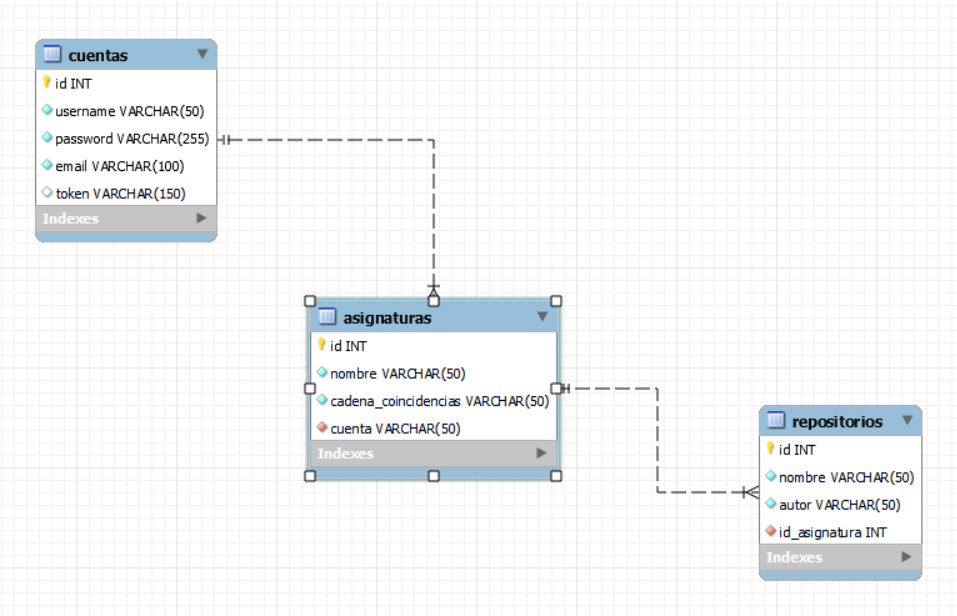
\includegraphics[width=1\textwidth]{DDBBSchema.png}
  \caption{Esquema entidad-relación de la aplicación desarrollada.}
  \label{figure:MySQLDraw}
\end{figure}

Mediante la implementación del servidor web y el servicio de persistencia,
podríamos obtener una solución viable y funcional. Sin embargo, es
conveniente, en este caso, separar el servidor web de la consulta de datos
al servicio de GitHub. El servidor web está destinado al múltiple acceso de
los usuarios, sobre el cual requerimos de un buen rendimiento y tiempo de
respuesta, lo que puede verse afectado por la gestión de múltiples
peticiones a otro servicio.

Por consiguiente, se ha implementado un segundo servidor, también
desarrollado en NodeJS, el cual está encargado de realizar toda la
comunicación con los servidores de Github. De esta forma, contaremos con:

\begin{itemize}
\item \textbf{El primer servidor, web}, el cual implementa todo el
  servicio web, destinado únicamente a recibir y responder las peticiones
  web de los usuarios. Este servidor será por tanto el encargado de
  comunicarse con la base de datos y gestionarla, realizando las consultas
  de registro y creación de usuarios, así como gestionar las asignaturas.
  En caso de necesitar datos provenientes del API Rest de Github, estos
  datos se solicitan al segundo servidor.
\item \textbf{El segundo servidor, servidor proxy Rest sobre GitHub},
  implementa un servicio encargado de atender las peticiones del primer
  servidor e intercomunicarse con el API de GitHub para obtener los datos
  solicitados. Por tanto, actúa a modo de proxy para el servicio de GitHub.
\end{itemize}

\begin{figure}[h!]
  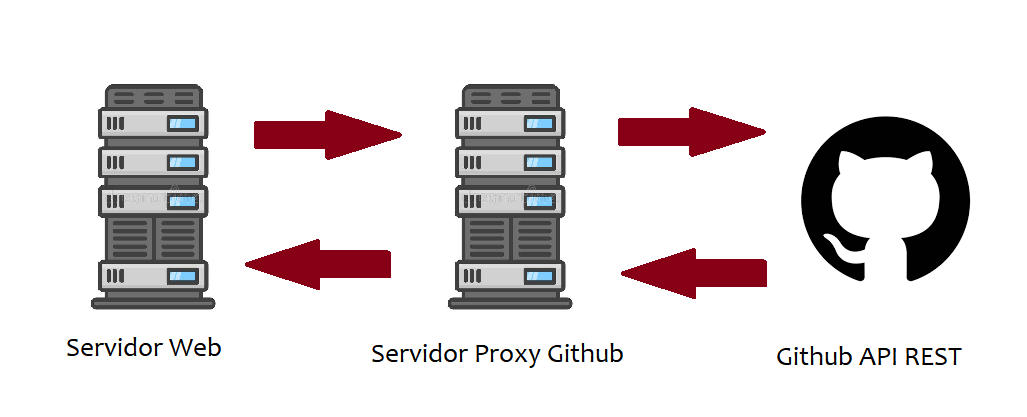
\includegraphics[width=1\textwidth]{Servidores.png}
  \caption{Grafico de funcionamiento de los servidores implementados y el
    servicio API de GitHub.}
  \label{figure:servidores}
\end{figure}

En la figura~\ref{figure:servidores}, se representa mediante un gráfico el
flujo de comunicación entre los servidores implementados y el API que
ofrece GitHub.

Respecto la comunicación de los dos servidores, el segundo servidor está
implementado a modo de API REST, donde recibe peticiones HTTP, en este caso
únicamente recibe peticiones de tipo GET, recibiendo por los parámetros de
la url los datos que se desean obtener. Una vez recibida la petición y
procesada, se comunica con el API de GitHub, obtiene los datos
correspondientes, y responde de nuevo al primer servidor.

\begin{figure}[h!]
  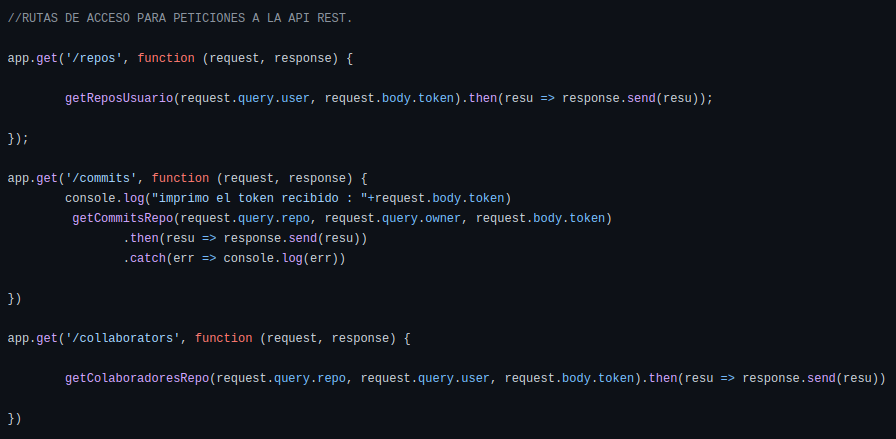
\includegraphics[width=\textwidth]{ProxyGitHub.png}
  \caption{Configuración del servidor proxy GitHub, implementación en
    NodeJS con Express.}
  \label{figure:ProxyGitHub}
\end{figure}

En la figura~\ref{figure:ProxyGitHub}, se muestran los diferentes métodos
GET y la forma de especificar que información se desea recuperar mediante
el uso de parametros en la url de la petición.


Como hemos comentado, las causas de la implementación del segundo servidor
es destinar únicamente el servidor web para los usuarios y no sobrecargarlo
con peticiones a otro servicio externo, reduciendo así su carga de trabajo
y mejorando los tiempos de respuesta. Además, conseguimos de esta forma,
separar la arquitectura de la aplicación, teniendo por una parte la
implementación del frontend, a la cual tienen acceso los clientes, y el
backend, encargado de proveer la información al frontend, de tal forma que
ambos servicios son independientes.
Posteriormente veremos que esta separación también permite distribuir mejor
la aplicación desarrollada sobre un servicio Cloud, permitiendo escalar
cada servicio en medida de la sobrecarga que se produzca.


\section{Consulta de datos al API de GitHub y autenticación}

Para la implementación de la aplicación se utiliza la librería
“Octokit”, una librería ofrecida de forma oficial
por el proveedor de servicios, y que se integra con el lenguaje Javascript.
Mediante ella, podemos realizar las consultas al API de Github de una
manera sencilla y teniendo acceso a operaciones de repositorios privados,
que requieren acceso mediante token. Con esta librería, las peticiones
realizadas se configuran con las cabeceras adecuadas para garantizar la
seguridad necesaria. Vemos a continuación un fragmento de código que
representa en Javascript la obtención de una instancia de la librería y una
función utilizada para recuperar la información de un usuario a través del
API proporcionada.


\begin{figure}[h!]
  \centerline{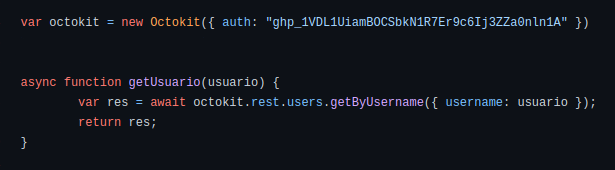
\includegraphics[width=1\textwidth]{octokit.png}}
  \caption{Ejemplo de uso de la librería Ocktokit, ofrecida por GitHub.}
  \label{figure:octokit}
\end{figure}

En la figura~\ref{figure:octokit} se muestra la creación e inicialización
de un objeto ``Octokit'', objeto ofrecido por la librería, mediante el cual
posteriormente se realizarán las peticiones HTTP, para su creación le
brindamos el token del usuario, necesario para poder leer la información de
sus repositorios.

En el caso de nuestro desarrollo, será el segundo servidor, el proxy a
GitHub, el que integrará la librería octokit a través de la cual se
autorizará al usuario mediante uso de token, pudiendo así recuperar los
datos del mismo. En el gráfico~\ref{figure:octokitGitApi}, encontramos una
visión del funcionamiento de la librería Octokit para la autorización y
posterior acceso a los datos.

\begin{figure}[h!]
  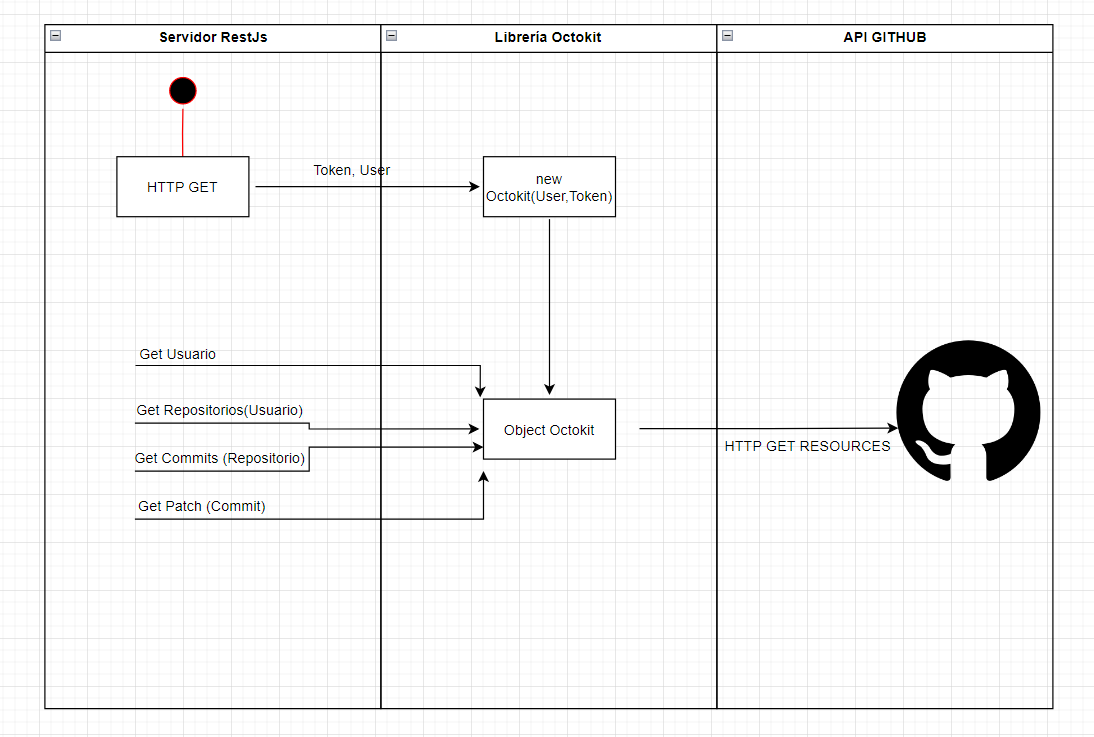
\includegraphics[width=1\textwidth]{OctokitGithubAPI.png}
  \caption{Gráfico de funcionamiento de la librería Octokit y peticiones al
    API REST de GitHub.}
  \label{figure:octokitGitApi}
\end{figure}


\section{Maquetado de la aplicación web}

La funcionalidad de la web debe ser, en un primer lugar, permitir registro
e inicio de sesión. Y en segundo lugar, mostrar los repositorios,
permitiendo el filtrado o bien por cadenas de caracteres, o bien por
filtrado en base a asignaturas previamente creadas por el usuario de la
aplicación.

Para la implementación de la web, se basa en cuatro vistas diferentes, dos
de ellas para registro e inicio de sesión, una para la página de inicio,
donde se muestran los repositorios y asignaturas del usuario, y por último
la página donde se visualizan las estadísticas del repositorio, esta última
accesible al hacer click sobre algún repositorio en la página principal.

Para el diseño de las vistas, se ha utilizado tecnologías específicas para
la tarea, dando estructura a las páginas con HTML, para posteriormente
añadir con CSS\cite{GradienteCSS} y Bootstrap\cite{Bootstrap} estilos, y
por último implementar animaciones y eventos en Javascript. Por otra parte,
para la creación de los gráficos, se ha utilizado una librería especificada
en Javascript, Chart.js\cite{ChartJS,ChartJSIntro}, permitiéndonos dibujar
gráficos y pudiendo añadirle animaciones y interacción con el usuario a los
mismos.

% En el caso de las páginas de inicio de sesión y estadísticas,
% al solicitar las webs al servidor, este nos envía la estructura y diseño de
% la web, además del código javascript asociado a la página, mediante el
% cual, se solicitarán de manera asíncrona, la información al servidor para
% completar las vistas. Por ejemplo, en el caso de acceder a la página
% principal, el servidor nos responde con una tabla vacía, que justo cuando
% se recibe, se realiza otra petición asíncrona al servidor que una vez
% resuelta, hará que los datos se muestren en el interior de la tabla.

El diseño de la web se ha implementado mediante funciones Javascript que se
ejecutarán una vez la página se haya cargado en el navegador, que
realizarán el completado de la vista con la información obtenida. De esta
forma, logramos que la respuesta a la petición sea inmediata, y
posteriormente cuando los datos sean recuperados se muestran. Así, el
usuario no percibe un retraso al acceder al sitio web, como ocurriría si
esperamos a enviar la web desde el servidor una vez los datos de GitHub se
hayan recuperado.

\section{Contenerización y despliegue de aplicación}

Uno de los objetivos del proyecto es ofrecer una implementación útil para
el despliegue en un servicio Cloud, de tal forma que los servicios estén
basados en contenedores que puedan ser lanzados en una estructura de nodos
cloud, permitiendo así su control y escalado. Por consiguiente, se ofrecen
junto el proyecto, las herramientas necesarias para formar contenedores con
cada uno de los servicios implementados. En primer lugar, una imagen Docker
para cada uno de los servidores Node, y un fichero docker-compose como
herramienta para simplificar el despliegue de ambos servidores en
Node, como un contenedor para la base de datos MySQL, configurado e
inicializado para funcionar de forma integrada con los otros servicios.

Estos contenedores, en caso de contar con un proveedor cloud, se pueden
desplegar y escalar, por ejemplo, usando para el propósito un orquestador
como podría ser Kubernetes, uno de los gestores de contenedores más popular
a día de hoy, permitiéndonos establecer configuraciones donde podríamos
lanzar los servicios y en caso de caída de alguno de ellos levantarse de
forma automática. Además, ofrece posibilidades como el escalado automático
en momentos donde la carga de trabajo está creciendo de manera paulatina,
repartiendo así la carga de trabajo y evitando el colapso.

Con la implementación de lo comentado, validaríamos el requisito de la
contenerización de la aplicación y la posibilidad de la integración del
proyecto sobre un entorno Cloud.

%\hilight{A continuación iría en el apéndice, y aquí diría que con lo
%  mostrado hasta ahora de contenedores se cumple el requisito de que la
%  aplicación fuera basada en contenedores}


%%% Local variables:
%%% TeX-master: "memoria.tex"
%%% coding: utf-8
%%% ispell-local-dictionary: "spanish"
%%% TeX-parse-self: t
%%% TeX-auto-save: t
%%% fill-column: 75
%%% End:

%  LocalWords:  NoSQL schemaless metadatos
